\section{Spectrometers}
The major experimental equipment in Hall C consists of two medium-resolution,
large-acceptance magnetic spectrometers with similar flexible detector
packages.
The High Momentum Spectrometer (HMS) is designed to analyze particles with
momenta up to \SI{7.4}{\giga\electronvolt}.
The Super High Momentum Spectrometer (SHMS) is designed to analyze particles
with momenta up to \SI{11}{\giga\electronvoltj}.
The spectrometers' detector packages are designed to analyze both electrons
and hadrons in coincidence or single-arm experiments studying inclusive and
exclusive reactions.
Both spectrometers' magnets and detector stacks sit on independent carriages
that rotate on rails around a central pivot located beneath the target chamber.
A summary of the spectrometers' performance is given in
table~\ref{tab:spectrometer_performance}.


For E12-06-102's production data, protons were detected in the SHMS in
coincidence with electrons in the HMS.
Additional single-arm data were taken for the purpose of detector calibration.

\begin{table}[h]
    \centering
    \caption{Summary of the HMS performance and design specifications for the SHMS.}
    \label{tab:spectrometer_performance}
    \resizebox{1.0\textwidth}{!}{
        \begin{tabular}[t]{lll}
            \hline
            \hline
            Parameter                            & HMS                            & SHMS                        \\
            \hline
            Central Momentum Range               & 0.4 \textendash 7.4 GeV/c      & 2 \textendash 11 GeV/c      \\
            Momentum Acceptance                  & $\pm10\%$                      & $-10\%$ to $+22\%$          \\
            Momentum Resolution                  & $0.1\%-0.15\%$                 & $0.03\%-0.08\%$             \\
            Scattering Angle Range               & 10.5$^\circ$ to 90$^\circ$     & 5.5$^\circ$ to 40$^\circ$   \\
                                                                                                                \\
            Target Length Accepted at 90$^\circ$ & 10 cm                          & 50 cm                       \\
            Horizontal Angle Acceptance          & $\pm32$ mrad                   & $\pm18$ mrad                \\
            Vertical Angle Acceptance            & $\pm85$ mrad                   & $\pm50$ mrad                \\
            Solid Angle Acceptance               & 8.1 msr                        & $>$4 msr                    \\
                                                                                                                \\
            Horizontal Angle Resolution (yptar)  & 0.8 mrad                       & 2 \textendash 4 mrad        \\
            Vertical Angle Resolution (xptar)    & 1.0 mrad                       & 1 \textendash 2 mrad        \\
            Target resolution (ytar)             & 0.3 cm                         & 0.2 - 0.6 cm                \\
                                                                                                                \\
            Maximum DAQ Event Rate               & 2000 events/second             & 10,000 events/second        \\
            Maximum Flux within Acceptance       & $\sim 5$ MHz                   & $\sim 5$ MHz                \\
                                                                                                                \\
            e/h Discrimination                   & $>$1000:1 at $98\%$ efficiency & 1000:1 at $98\%$ efficiency \\
            $\pi$/K Discrimination               & 100:1 at $95\%$ efficiency     & 100:1 at $95\%$ efficiency  \\
            \hline
        \end{tabular}
    } % resizebox
\end{table}

\subsection{High Momentum Spectrometer}
The HMS is a 25$^{\circ}$ vertical bend spectrometer with superconducting
magnets in a QQQD configuration.
Its maximum central momentum is \SI{7.4}{\giga\electronvolt} with an acceptance of $\sim\pm10\%$.
The HMS detector stack consisting of a hodoscope, lead glass calorimeter,
Cherenkov counter, and pair of drift chambers sits in a concrete shielding
hut approximately 27 m from the target chamber.
A vacuum is maintained in the region between the entrance to Q1 and
the dipole exit to minimize multiple scattering.

\begin{figure}[!ht]
    \centering
    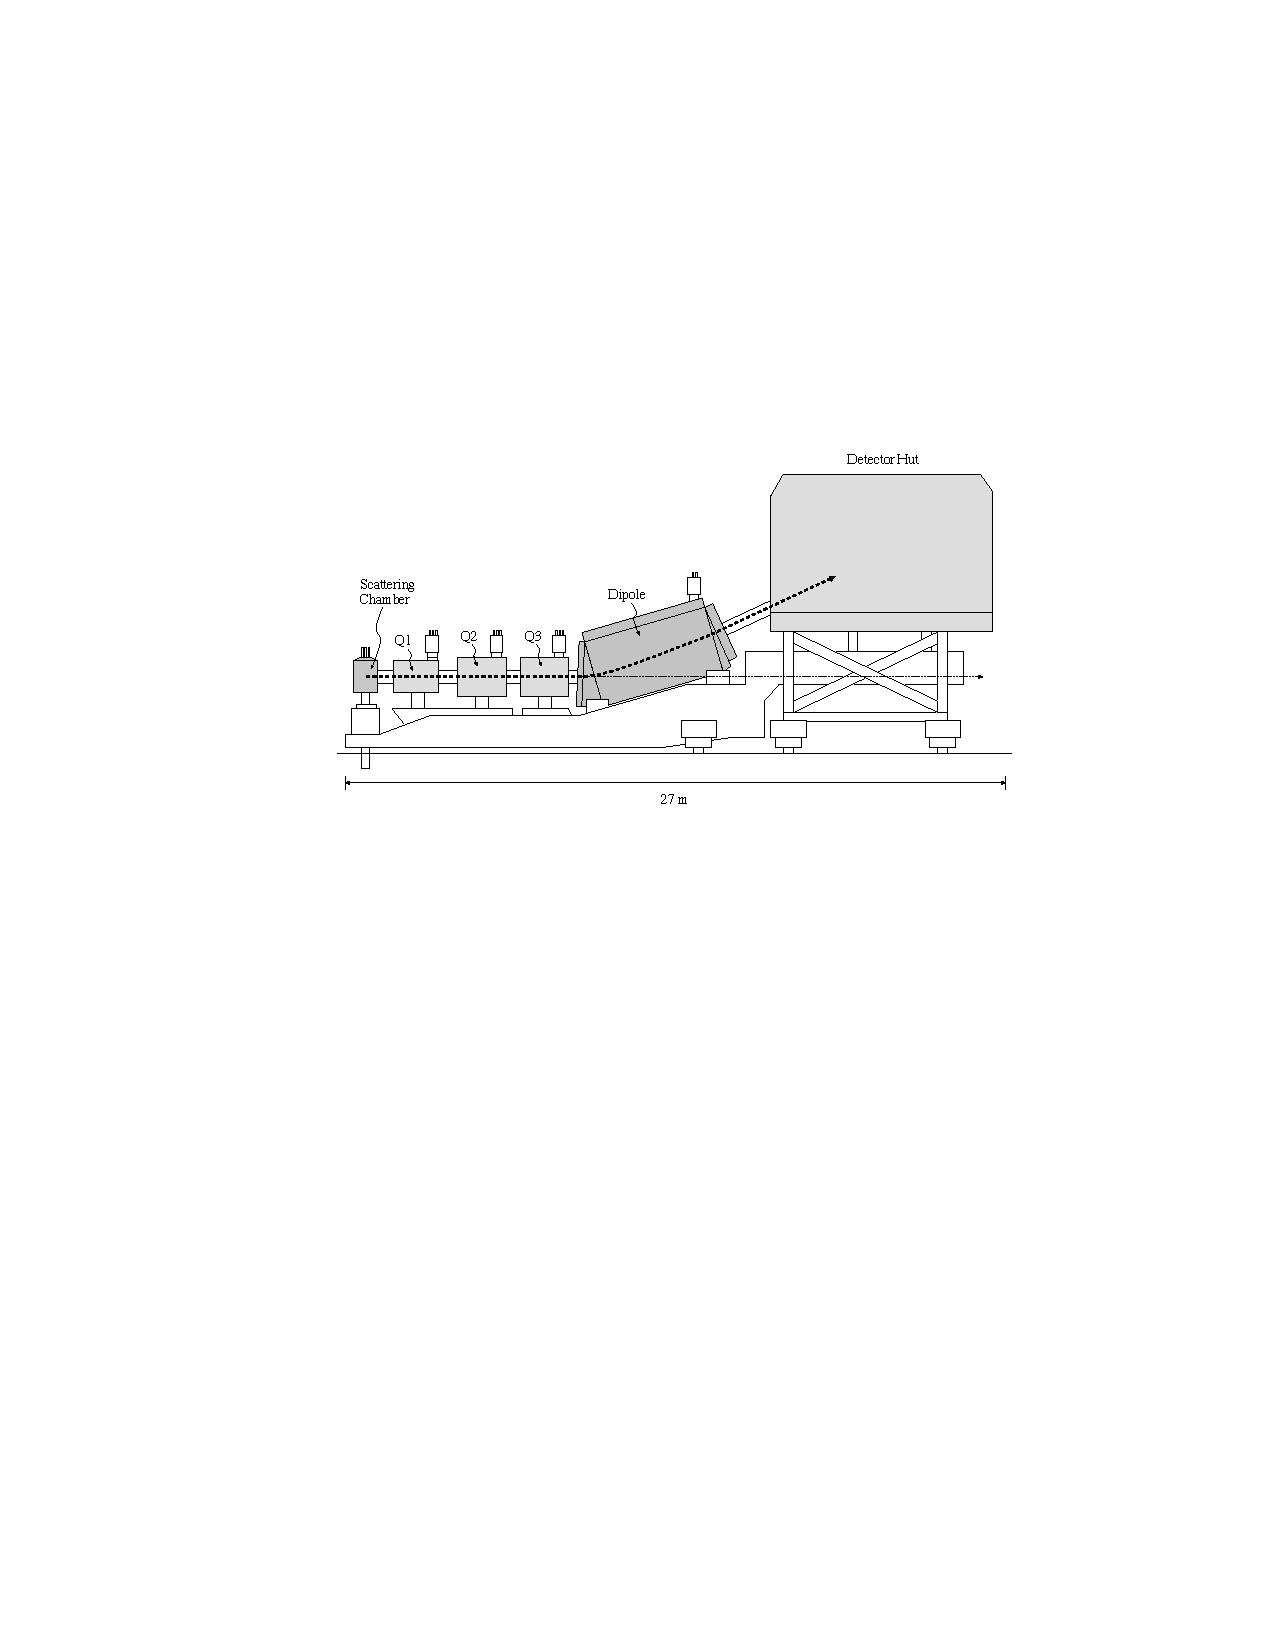
\includegraphics[width=1.0\textwidth]{chap3/hms_schematic.pdf}
    \caption{High Momentum Spectrometer (HMS) side view.}
    \label{fig:hms_schematic}
\end{figure}

The HMS's performance is well understood from \SI{6}{\giga\electronvolt} era experiments, but
some changes have been made for the \SI{12}{\giga\electronvolt} era.
The dipole NMR probe was moved outside the dipole for more accurate measurement
of central momenta.
The original HMS drift chambers were replaced with a pair of drift chambers
that match the design of those in the SHMS.

Optics calibration runs\footnote{HMS singles with run numbers 1337–1352}
using hydrogen elastic scattering and carbon data were taken to determine
central dipole field values, external NMR measurements, and corresponding
magnet currents.
These data were also used to characterize spectrometer mispointing and angular
offsets and optimize the matrix used in projecting tracks from the focal
plane to the interaction at the target.
See \cite{Holly_HMS_Optics} for more details.

\subsection{Super High Momentum Spectrometer}
Like the HMS, the SHMS is an 18.4$^{\circ}$ vertical bend spectrometer with
superconducting magnets in a QQQD configuration.
To allow it to reach smaller scattering angles, the SHMS has an additional
3$^{\circ}$ horizontal bender (HB) dipole before the first quadrupole.
Its maximum central momentum is 11 GeV with an acceptance covering $-10\%$
to $+22\%$.
The SHMS detector stack consisting of a hodoscope, lead glass calorimeter,
three Cherenkov counters, and pair of drift chambers sits in a concrete
shielding hut approximately 22 m from the target chamber.

\begin{figure}[!ht]
    \centering
    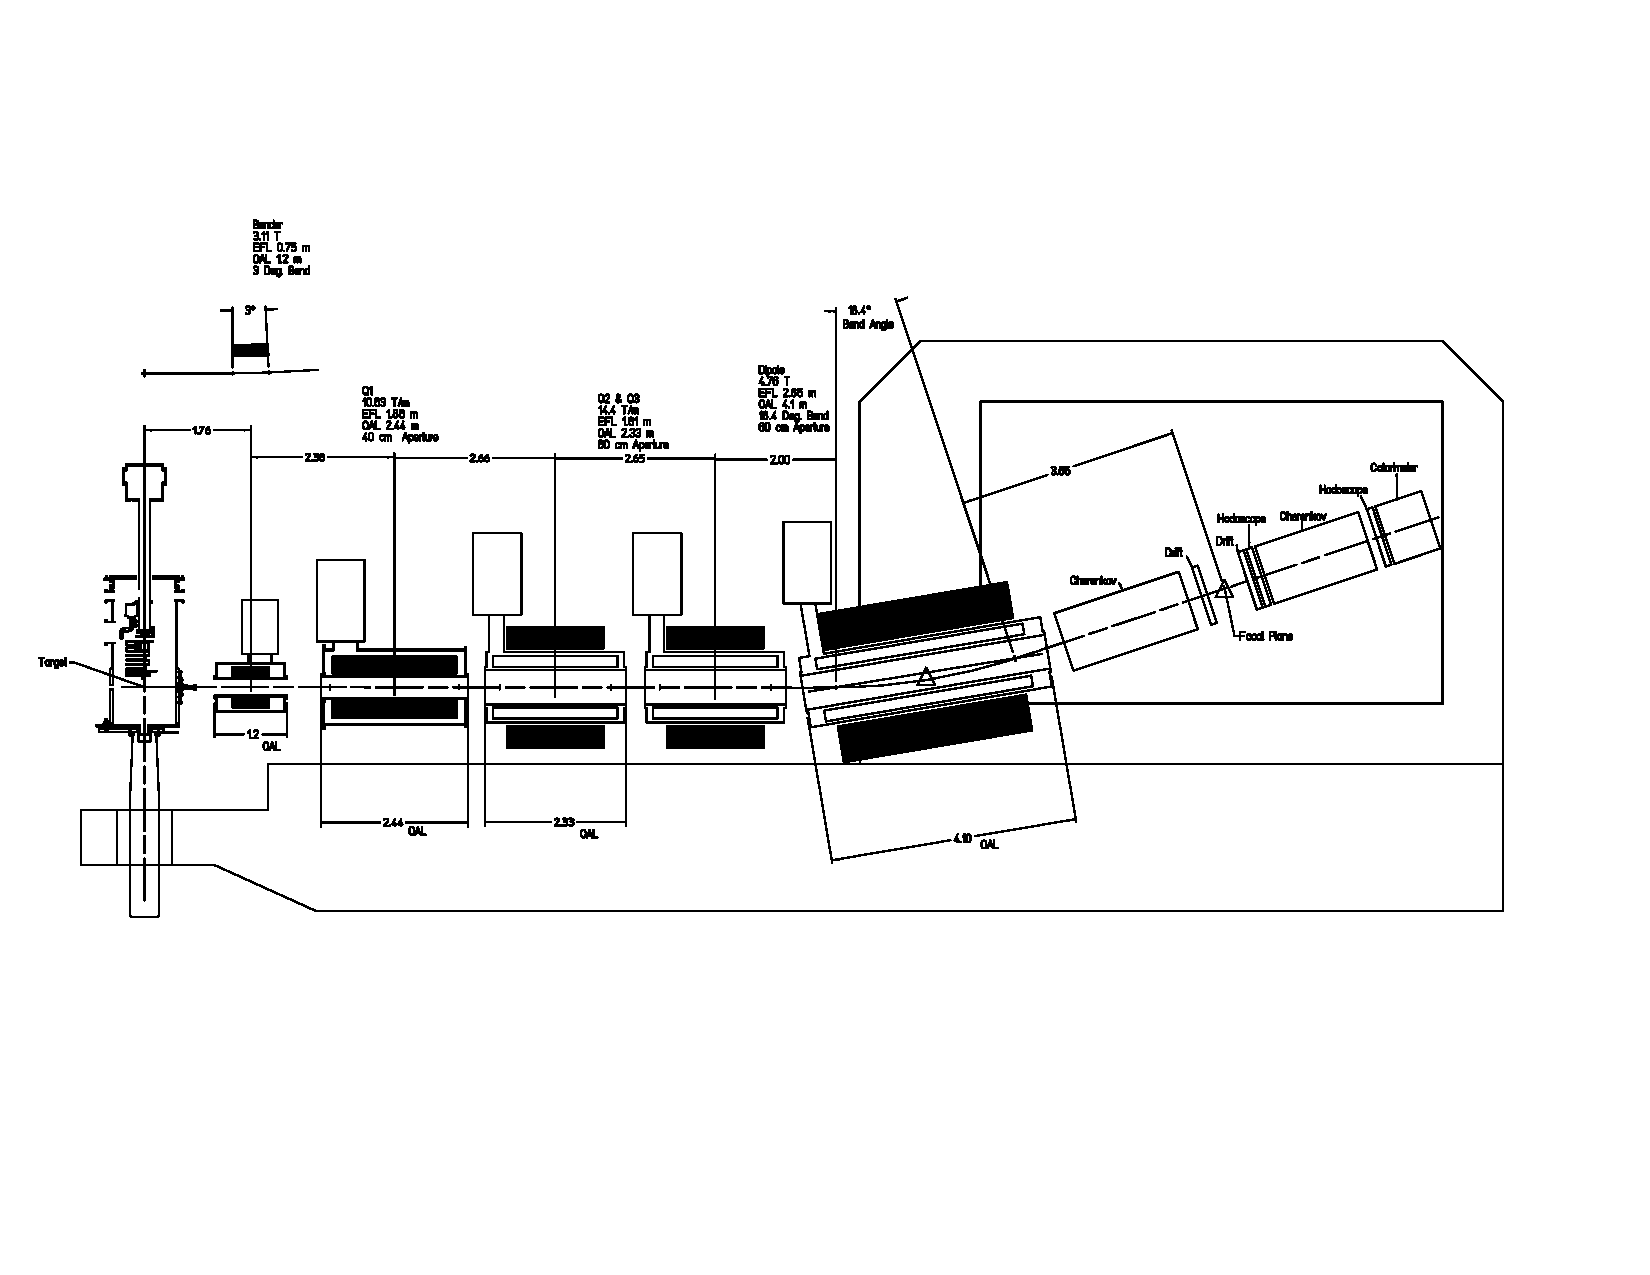
\includegraphics[width=1.0\textwidth]{chap3/SHMS_Layout_new.pdf}
    \caption{Super High Momentum Spectrometer (SHMS) side view.}
    \label{fig:shms_schematic}
\end{figure}

As with the HMS, she commissioning of the SHMS magnets used hydrogen and carbon
elastic scattering and the 4.4 MeV carbon excited peak to characterize
spectrometer mispointing and angular offsets and optimize the track
reconstruction matrix.
See \cite{Holly_SHMS_Optics} for more details.

\subsection{Collimators and Slit Systems}
The HMS has a remotely operated collimator ladder installed on the front face
of Q1.
The HMS ladder contains one sieve-slit for optics tuning and two
solid-angle-defining collimators.

The SHMS has a similar system installed on the front face of Q1.
The SHMS ladder contains two sieve-slits for optics tuning and one
solid-angle-defining collimator.
The two sieve slits consist of a lattice of holes separated by 0.6457"
horizontally and 0.9843" vertically.
Two holes in each sieve are missing to ensure correct orientation.
To account for the HB magnet, the SHMS has an additional sieve slit ladder
placed immediately upstream from the HB.
